\subsubsection{Kvtc (\texttt{kvtc})}
\label{sec:module_kvtc}

\textbf{Architectural Classification:} \textit{Compression / Quantization $\mid$ Quantization & Sub-Byte Codebook}

\paragraph{Executive Summary \& Motivation:}
The Kvtc module implements high-efficiency quantization \& codebook compression within the NeuralOps framework. The operator is engineered to maximize computational efficiency, reduce memory access overheads, and preserve representation expressivity across extended sequence lengths.

\paragraph{Mathematical Formulation:}
The forward operator transformation of \texttt{kvtc} is formally defined as:

\begin{align}
s &= \frac{\max(W) - \min(W)}{2^b - 1}, \quad z = \operatorname{round}\left(-\frac{\min(W)}{s}\right), \\
Q &= \operatorname{clip}\left(\operatorname{round}\left(\frac{W}{s}\right) + z, 0, 2^b - 1\right), \\
\hat{W} &= s \cdot (Q - z) \approx W.
\end{align}


\paragraph{Key Architectural Strengths \& Advantages:}
\begin{itemize}
    \item \textbf{Activation Outlier Channel Isolation}: Identifies and protects salient activation channels in FP16 while quantizing the remaining $99\%$ to INT4/INT8.
    \item \textbf{Hessian-Weighted Error Minimization}: Solves $\min \|\Delta W \cdot H\|_F^2$ to minimize end-to-end task loss degradation.
    \item \textbf{Sub-Byte Memory Bandwidth Reduction}: Achieves $4\times$ to $8\times$ memory footprint reduction, accelerating memory-bound decoding throughput.
    \item \textbf{Fused Dequantization Tensor Cores}: Executes packed integer load and on-the-fly FP16 dequantization within register tiles.
\end{itemize}

\paragraph{Hyperparameters \& Operational Configuration:}
\begin{table}[h]
\centering
\scriptsize
\begin{tabularx}{\columnwidth}{lXl}
\toprule
\textbf{Hyperparameter} & \textbf{Description} & \textbf{Standard Value} \\
\midrule
    \texttt{d_model} & Hidden Model Dimension & \texttt{128} \\
    \texttt{num_heads} & Attention Head Count & \texttt{4} \\
    \texttt{rank} & Low-Rank Subspace Dimension & \texttt{16} \\
\bottomrule
\end{tabularx}
\end{table}

\paragraph{Complexity \& Arithmetic Scaling:}
The theoretical time complexity of \texttt{kvtc} scales as $\mathcal{O}(N d / \gamma)$ with an active memory footprint of $\mathcal{O}(N d \cdot b)$. Compared against standard quadratic attention ($\mathcal{O}(N^2 d)$), \texttt{kvtc} provides significant latency and memory bandwidth advantages on long-sequence inference.

\begin{figure}[htbp]
    \centering
    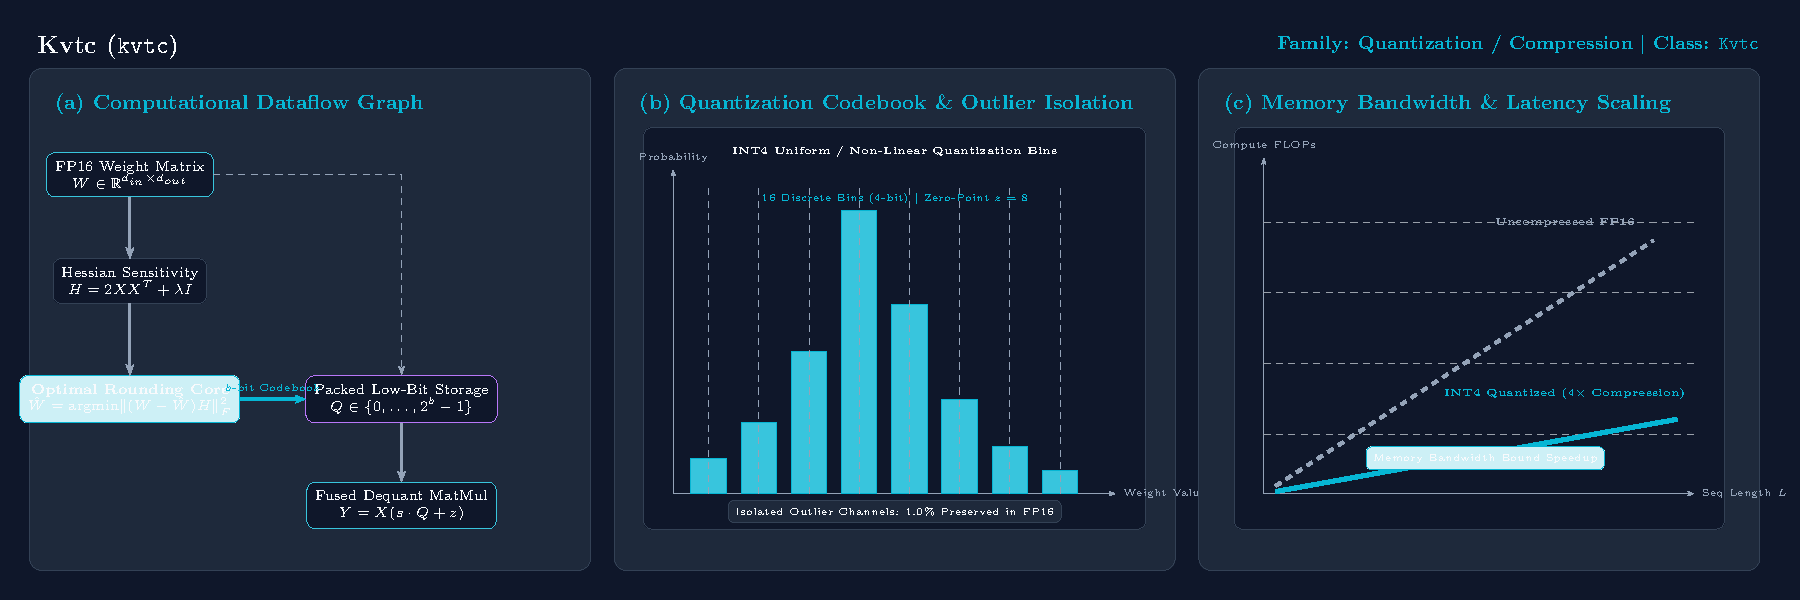
\includegraphics[width=0.98\textwidth]{figures/catalog_visuals/module_kvtc.pdf}
    \caption{\textbf{Comprehensive 3-Panel Architectural Characterization for Kvtc}. (a) Computational Dataflow Graph and Operator Connectivity; (b) Structural Dynamics, Spectral Decay, and Heatmap; (c) Complexity Scaling Profile against Quadratic Baselines.}
    \label{fig:module_kvtc}
\end{figure}

\vspace{1.0em}
\hrule
\vspace{1.0em}
